One of the main ideas in complex systems is emergence. Emergence means that the structure of the particles is simple and they are not so important like interactions bettween them. \\
An example of this is the Central limit theorem, which comes from mathematics. \\ \\
If you have a random variable $x_k$, with average value $\lang x_k \rang = 0$ and finite variance $\sigma^2$, then the central limit theorem says that, if the variables are independent (and in physics this is usally a fair assumption) for every value of $k$, then the normalized sum 
$$
	z_n = \frac{1}{\sqrt{N}}\sum_{k=0}^N x_k
$$
then the distribution of this variable $z_n$ is known, and it is gaussian, for a big enough value of $N$.
$$
	\rho(z_n) \sim \exp\left(-\frac{z^2}{2\sigma^2}\right)
$$
Despite the fact that we, as humans, need a cause-effect relationship to describe a phenomenon, nature loves independent events, like DNA mutations.
The gaussian describes the fluctuations of a system at equilibrium, not the complexity. You cannot extract work from fluctuations at equilibrium, otherwise you violate thermodynamics (and that's no good). \\
The gaussian function is not a physical function, because it implies non zero probabilities to events which are impossible. For example, if we take a particle in a basin of attraction of a potential, the non zero probability given by the gaussian fluctuations allows the particle to jump out of the pit. But this violates the second law of thermodynamics. \\ \\
A way to defy the gaussian properties is to allow a system to have memory, so to remove the independence of the variable. 
\begin{center}
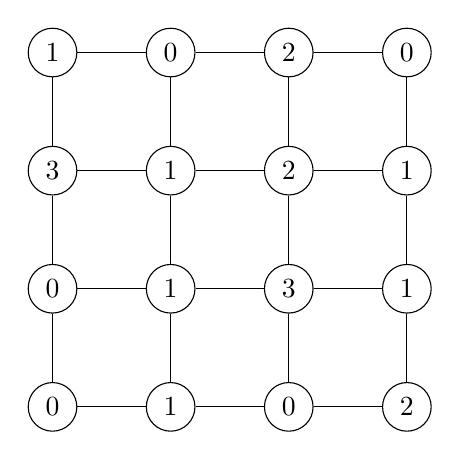
\begin{tikzpicture}[node distance={15mm}, main/.style = {draw,circle}]
\node[main] (1) {1};
\node[main] (2) [right of=1] {0};
\node[main] (3) [right of=2] {2};
\node[main] (4) [right of =3] {0};
\node[main] (5) [below of =1] {3};
\node[main] (6) [right of=5] {1};
\node[main] (7) [right of=6] {2};
\node[main] (8) [right of=7] {1};
\node[main] (9) [below of=5] {0};
\node[main] (10) [right of=9] {1};
\node[main] (11) [right of=10] {3};
\node[main] (12) [right of=11] {1};
\node[main] (13) [below of=9] {0};
\node[main] (14) [right of=13] {1};
\node[main] (15) [right of=14] {0};
\node[main] (16) [right of=15] {2};
\draw (1) -- (2);
\draw (1) -- (5);
\draw (2) -- (3);
\draw (3) -- (4);
\draw (5) -- (6);
\draw (6) -- (7);
\draw (7) -- (8);
\draw (5) -- (9);
\draw (9) -- (10);
\draw (10) -- (11);
\draw (11) -- (12);
\draw (9) -- (13);
\draw (13) -- (14);
\draw (14) -- (15);
\draw (15) -- (16);
\draw (2) -- (6);
\draw (3) -- (7);
\draw (4) -- (8);
\draw (6) -- (10);
\draw (7) -- (11);
\draw (8) -- (12);
\draw (10) -- (14);
\draw (11) -- (15);
\draw (12) -- (16);
\end{tikzpicture}
\end{center}
One example of this is the sand pile model. You have a lattice, and each point is connected to its four neighbors. At this point one particle is put in a randomly chosen point. Each node can have four possible states, $0,1,2,3$, that is four possible numbers of particles. If a node reaches 4 particles, the 4 particles are distributed to the 4 neightbouring nodes.
\begin{center}
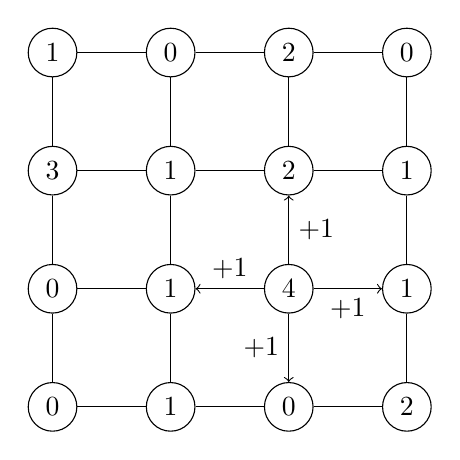
\begin{tikzpicture}[node distance={15mm}, main/.style = {draw,circle}]
\node[main] (1) {1};
\node[main] (2) [right of=1] {0};
\node[main] (3) [right of=2] {2};
\node[main] (4) [right of =3] {0};
\node[main] (5) [below of =1] {3};
\node[main] (6) [right of=5] {1};
\node[main] (7) [right of=6] {2};
\node[main] (8) [right of=7] {1};
\node[main] (9) [below of=5] {0};
\node[main] (10) [right of=9] {1};
\node[main] (11) [right of=10] {4};
\node[main] (12) [right of=11] {1};
\node[main] (13) [below of=9] {0};
\node[main] (14) [right of=13] {1};
\node[main] (15) [right of=14] {0};
\node[main] (16) [right of=15] {2};
\draw (1) -- (2);
\draw (1) -- (5);
\draw (2) -- (3);
\draw (3) -- (4);
\draw (5) -- (6);
\draw (6) -- (7);
\draw (7) -- (8);
\draw (5) -- (9);
\draw (9) -- (10);
\draw[->] (11) -- node[above]{+1} (10);
\draw[->] (11) -- node[below]{+1} (12);
\draw (9) -- (13);
\draw (13) -- (14);
\draw (14) -- (15);
\draw (15) -- (16);
\draw (2) -- (6);
\draw (3) -- (7);
\draw (4) -- (8);
\draw (6) -- (10);
\draw[->] (11) -- node[right]{+1} (7);
\draw (8) -- (12);
\draw (10) -- (14);
\draw[->] (11) -- node[left]{+1} (15);
\draw (12) -- (16);
\end{tikzpicture}
\end{center}
\begin{center}
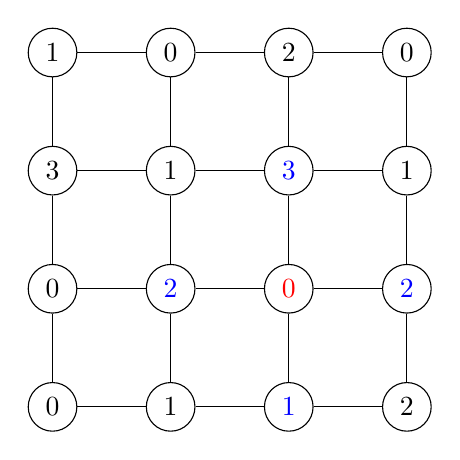
\begin{tikzpicture}[node distance={15mm}, main/.style = {draw,circle}]
\node[main] (1) {1};
\node[main] (2) [right of=1] {0};
\node[main] (3) [right of=2] {2};
\node[main] (4) [right of =3] {0};
\node[main] (5) [below of =1] {3};
\node[main] (6) [right of=5] {1};
\node[main] (7) [right of=6] {\textcolor{blue}{3}};
\node[main] (8) [right of=7] {1};
\node[main] (9) [below of=5] {0};
\node[main] (10) [right of=9] {\textcolor{blue}{2}};
\node[main] (11) [right of=10] {\textcolor{red}{0}};
\node[main] (12) [right of=11] {\textcolor{blue}{2}};
\node[main] (13) [below of=9] {0};
\node[main] (14) [right of=13] {1};
\node[main] (15) [right of=14] {\textcolor{blue}{1}};
\node[main] (16) [right of=15] {2};
\draw (1) -- (2);
\draw (1) -- (5);
\draw (2) -- (3);
\draw (3) -- (4);
\draw (5) -- (6);
\draw (6) -- (7);
\draw (7) -- (8);
\draw (5) -- (9);
\draw (9) -- (10);
\draw (11) -- (10);
\draw (11) -- (12);
\draw (9) -- (13);
\draw (13) -- (14);
\draw (14) -- (15);
\draw (15) -- (16);
\draw (2) -- (6);
\draw (3) -- (7);
\draw (4) -- (8);
\draw (6) -- (10);
\draw (11) -- (7);
\draw (8) -- (12);
\draw (10) -- (14);
\draw (11) --  (15);
\draw (12) -- (16);
\end{tikzpicture}
\end{center}
For the nodes in the border, what happens is that 2 of the particles are redistributed and the other 2 are released in the enviroment, so they are lost. \\ \\
So this system has memory, and this means that the states of all the nodes are not independent. This memory turns the gaussian distribution into a power law
$$
	p(n) \propto n^{-\alpha}
$$
with $\alpha > 1$. \\
The decay of the power low is much slower than that of the gaussian, which means that the probability to have events in the extremes is significantly higher with the power low distribution.
Memory is related to power laws, but vice versa is not guaranteed.
We can also have power laws in physics, for example in the Ising model.
In physics, power laws typically represent a phase transition for a dynamic system in a non-equilibrium state. \\
In the sand pile model, we notice a self-organized criticality: the system naturally goes into a critical state and does a phase transition. \\
Another example of a natural power law is the Kleiber law which relates the metabolic rate (amount of energy you need to survive) to the mass.
\begin{equation}
	E(m) \propto m^{\frac{4}{3}}
\end{equation}
We can also observe that heartbeat rate decreases with mass and lifetime increases.
\section{Total energy in a network}